\documentclass[10pt]{article}
\usepackage[a4paper,margin=21mm,top=18mm,bottom=21mm]{geometry}
\usepackage{amsmath,amssymb,amsthm,graphicx,booktabs,xcolor,hyperref,fancyhdr}
\definecolor{ink}{HTML}{194E53}\definecolor{mut}{HTML}{51676A}\hypersetup{colorlinks=true,linkcolor=ink,urlcolor=ink}
\pagestyle{fancy}\fancyhf{}\renewcommand{\headrulewidth}{0pt}\renewcommand{\footrulewidth}{.3pt}\fancyfoot[L]{\footnotesize\sffamily\color{mut}ORDINARY SQUARE GRID\quad /\quad CONSTRUCTION UPDATE}\fancyfoot[R]{\sffamily\thepage}
\setlength{\parindent}{0pt}\setlength{\parskip}{5pt}\newcommand{\tagline}[1]{{\small\sffamily\bfseries\color{ink}#1}\par}\newcommand{\head}[1]{{\Large\sffamily\bfseries\color{ink}#1}\par}\newcommand{\sub}[1]{\par\smallskip{\large\sffamily\bfseries\color{ink}#1}\par}\newcommand{\F}{\mathbb F_p}\newcommand{\Z}{\mathbb Z}\newcommand{\htf}{F_{\rm ht}}\newcommand{\file}[1]{\texttt{\detokenize{#1}}}
\begin{document}
\tagline{RESEARCH NOTE\hfill 19 NOVEMBER 2026}
{\LARGE\sffamily\bfseries More points on the same board}\par
A \emph{cap} is a subset of $\{0,\ldots,n-1\}^2$ with no three distinct points on an ordinary straight line. All comparisons below use the same side $n$. A gain in the size of a construction need not be a literal addition to a fixed point set.
\sub{Finite comparisons with public witnesses}
\begin{center}\begin{tabular}{r r r r r r}\toprule
Side & Public [1] & Previous here & \textbf{New} & Gain vs public & Gain vs previous\\\midrule
16,018&24,306&24,469&\textbf{24,588}&282&119\\32,002&48,421&48,661&\textbf{48,838}&417&177\\64,006&96,816&97,008&\textbf{97,062}&246&54\\\bottomrule\end{tabular}\end{center}
For example the middle construction drops 1,092 points of the public witness and introduces 1,509 different ones. The net gain is 417. These are verified lower bounds, not proofs of unrestricted board optima or priority over every other construction.
\sub{Finite comparisons with our preceding half-turn sets}
\begin{center}\begin{tabular}{r r r r l}\toprule Side&Previous&\textbf{New}&Gain&Symmetry retained\\\midrule
293&446&\textbf{508}&62&quarter-turn\\389&594&\textbf{668}&74&quarter-turn\\4,037&6,176&\textbf{6,296}&120&half-turn\\10,085&15,364&\textbf{15,520}&156&half-turn\\\bottomrule\end{tabular}\end{center}
\begin{center}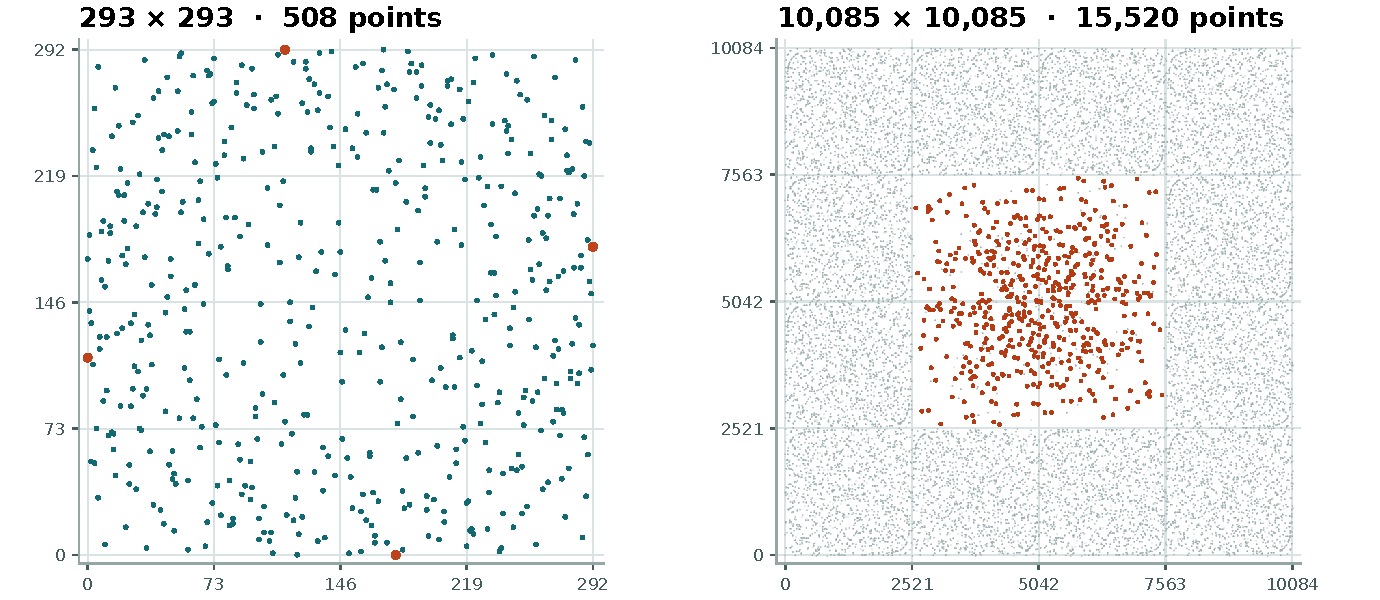
\includegraphics[width=.95\linewidth]{figures/two-caps.pdf}\end{center}
\small Left: one of 127 four-point orbits is highlighted. Right: gray points are retained from the 15,364-point set; orange marks the 544 additions (388 old points were dropped). Neither picture is a simulated density plot. The comparison at 293 is to our earlier set, not a 62-point gain over the literature: cropping one of the public side-300 witnesses in [2] already gives 504 there.\normalsize

\sub{What transfers to other grid sizes?}
The 48,838-point witness alone gives more than $3n/2$ on \emph{every} side from 31,669 through 32,558: embed it for $n\ge32,002$, or trim $32,002-n$ rows and as many columns, losing at most two points per deleted row or column. This is a finite interval. For unbounded sides the different construction on pages 3--5 improves the uniform half-turn guarantee by four points, from $2n-2p-16$ to $2n-2p-12$, whenever $p>3$ is prime and $3p\le n\le4p$.

\newpage\tagline{01\quad /\quad HOW TO BUILD AND CHECK THE EXAMPLES}\head{Adding versus replacing}
Let $p$ be one of $8009,16001,32003$, $n=2p$, $h=(p-1)/2$ and $J=\{h+1,\ldots,h+p\}$. Start with the translated Hall--Jackson--Sudbery--Wild frame of [1,3],
\[
 O=\{(x,y)\in[0,2p-1]^2\cap\Z^2:x(y-h)=1\pmod p\}\setminus J^2.
\]
It contains $3(p-1)$ points. Our compact certificate \file{data/final-P.txt} lists $p$, the number of deletions and the number of insertions on the first line, then the deletion coordinates followed by the insertion coordinates. The letter P stands for the decimal prime. This plus the formula specifies the whole construction, without rerunning a search.
\begin{center}\begin{tabular}{rrrrrr}\toprule
$p$ & Frame & Drop from frame & Insert into frame & Drop from public & Insert vs public\\\midrule
8009 &24,024 &580 &1,144 &660 &942\\16001 &48,000 &966 &1,804 &1,092 &1,509\\32003 &96,006 &1,015 &2,071 &1,157 &1,403\\\bottomrule\end{tabular}\end{center}
\sub{If not one public point may move}
Start instead with $O$ \emph{and all the published additions} in [1], \S8. Append the following zero-based points:
\begin{center}\begin{tabular}{rl}\toprule Side & Points to append simultaneously\\\midrule
16,018 & $(0,4140),(0,4259)$\\32,002 & $(0,8619),(0,9094),(13484,8000)$\\64,006 & $(0,16208),(0,16387),(35817,16001),(36424,16001)$\\\bottomrule\end{tabular}\end{center}
These give $24,308$, $48,424$ and $96,820$ respectively. The first two literal increments, 2 and 3, are sharp for the specified public sets. The exhaustive full-board lists of sites individually free against $O$ have sizes 388 and 614. After excluding the published additions and testing every surviving site against the full public set, the first board has only six possible sites, all on $x=0$. The second has eight on $x=0$ and only $(13484,8000)$ elsewhere. Hence at most two or three additions can coexist. On the third board we checked all four missing modular axes of $O$ and a separate central pool, \emph{not} every site on the board; four is a lower bound. In each case the displayed additions were checked together, not just one at a time.
\sub{Search and independent verification}
For the exchange search, pool the frame points with previously added sites and candidates meeting few frame secants. Group equal primitive directions from each candidate. Every line on at least three pool points must either pass through a candidate or have been a forbidden frame triple already. Impose capacity two on each such line. The search makes swaps between occupied and unoccupied sites; at two sides its pool is enlarged when earlier swaps release a blocked candidate. A different search on medium boards makes the quarter-turn orbit the unit of a move. At side 293 a single orbit is $(0,114),(178,0),(292,178),(114,292)$. Rotating all pairs in \file{data/orbits293.csv} by $0,90,180,270$ degrees gives the exhibited 508 points.

The independent checker uses exact integers. In the frame, a primitive physical line meets the reduced conic in at most two residues; a triple must contain two points of the same residue, of axis or unit-diagonal direction. Check those four directions on the retained frame. From \emph{each} insertion, compare primitive unoriented directions to every other final point. Equality is exactly a collinear triple. For the four rotational examples we instead checked every direction from every point, without assuming a carrier: 281,191,312 directions in total, also checking symmetry, distinctness and bounds.

\newpage\tagline{02\quad /\quad A UNIFORM IMPROVEMENT}\head{Fewer lost points in the general construction}
Let $\htf(n)$ be the maximum size with symmetry under $(x,y)\mapsto(n-1-x,n-1-y)$. Put $d=4p-n$ and $U=2n-2p-4$ for odd $n$, $U=2n-2p-6$ for even $n$.

\textbf{Theorem.} For every prime $p>3$ and every $3p\le n\le4p$, $\htf(n)\ge U-\delta$, where one may take
\[
\delta=\begin{cases}0 & p\equiv1\pmod{12},\\4 & p\equiv5\pmod{12},\\4 & p\equiv3\pmod4,\quad d\ge19,\\6 & p\equiv3\pmod4,\quad d<19.\end{cases}
\]
In particular the previous worst-case guarantee $2n-2p-16$ becomes $\mathbf{2n-2p-12}$. The previous zero-loss result for $d\ge32\sqrt p$ still applies. This is an additive improvement, not a change of density coefficient. For instance $p=2003,n=8012$ gives $12,006$ rather than the preceding generator's $12,002$; here $c=1399,t=1672$ in the formulas below. Taking the first prime $p\ge n/4$ applies the theorem to every sufficiently large $n$. More explicitly, for consecutive large primes $p<q$ and $4p\le n\le4q$, the bound is at least $3n/2-3(q-p)/2-12$: centre a side $4p$ or $4p-1$ construction of the appropriate parity, or use the theorem at $q$, and take the larger of $6p-12$ and $2n-2q-12$.
\sub{Inputs from the preceding construction}
We give the repair proof; the elementary construction lemmas used here are proved in [4, \S3], supplied with this note. The original six-site masks and signed-coset colouring are prior work [5]. Set $2\alpha=n-1\pmod p$, and use $(x-\alpha)(y-\alpha)=c\pmod p$. Fibre $u$ has residues $\alpha+u,\alpha+c/u$ and an array of $w\times k$ lifts, $w,k\in\{3,4\}$, indexed from its least $x,y$ by steps of $p$. Select lifts of a fixed physical parity $x+y$ in each signed class $[u]=\{u,-u\}$; choose the negatives by reflecting in the actual board centre. Allowed nonaxis repeated directions are
\[
 (1,\pm1),\quad (3,\pm1),\quad (1,\pm3).
\]
Their possible second residue is $u'=-ac/(bu)$ for direction $(a,b)$. Opposite physical parity excludes it. A tangent $u'=u$ cannot supply a second residue. An ordinary rectangular mask has $w+k-2$ points of the chosen parity; suppressing either high family $(3,\pm1)$ or $(1,\pm3)$ costs at most one point per fibre. In $3\times3$ both high families are absent at no cost. The nominal sum is exactly $U$, since the one missing coordinate residue occupies three columns for odd $n$ and four for even $n$, and likewise for rows. In $4\times4$ the standard even/odd sheet masks, both invariant under transposition, are
\[
 M_0=\{00,02,13,20,31,33\},\qquad M_1=\{01,03,10,23,30,32\}.
\]
The residue case $p=1\pmod{12}$ is already lossless in [4]. Otherwise let $K=\langle[3]\rangle$ in $\F^*/\{\pm1\}$, $L=|K|$, and choose a scale $t\ne0$. The involution $g\mapsto[c]/g$ pairs distinct cosets of $K$ except for $[t]K$; give paired cosets opposite colours. This holds because the quotient has odd order: for $p=3\pmod4$ even the full group has odd order; for $p=5\pmod{12}$ the nonsquare 3 generates the full 2-part in the cyclic signed group. In $[t]K$ index $[3^it]$ by $i\in\Z/L$. If $p=5\pmod{12}$ choose $c=t^2/3$, $L=2h$; colour the two half intervals oppositely. For partner maps $i\mapsto-1-i+s$, $s=0,\pm1$, the only defects are high-direction fixed signed vertices $0,h,h-1,-1$. They form two reciprocal pairs. If $p=3\pmod4$, choose $c=t^2$, $L=2h+1$, colour $0,\ldots,h$ one and $-h,\ldots,-1$ zero. The maps are $i\mapsto-i+s$. The defects are the positive diagonal at zero, the high edge $\{0,1\}$ and one high fixed direction at each of $h,-h$. Both lists follow by substitution. At a high fixed signed vertex only the direction whose actual partner is $-u$ needs attention; the other sign is tangent.

\newpage\tagline{03\quad /\quad THE LOCAL REPAIR}\head{Use the actual intercept, not just the slope}
Write $C=(n-1)/2$ as a real number. Represent the residue coordinate $u$ by an integer $v\equiv2u\pmod p$ of parity $n-1$. The lifts in that coordinate are $C+v/2+i p$ with $|v+2pi|\le4p-d-1$. Consequently $|v|<d$ gives three lifts, and
\[
 d<v<2p-d\ \Longrightarrow\ i=-2,-1,0,1.\tag{1}
\]
Replacing $v$ by $-v$ reverses the index list; increasing it by $2p$ subtracts one from every index.

\textbf{Away from the endpoint ($d\ge19$).} Set $2t=3z\pmod p$, taking $z=1$ or $2$ of the required parity. The coordinates $\pm t,\pm3t,\pm t/3$ now have three lifts, since $|z|,|3z|,|9z|<d$. For $p=5\pmod{12}$ the reciprocal vertices with coordinates $t,t/3$ therefore have no high defect; suppress one family at each of the other two signed vertices. The total loss is at most four. For $p=3\pmod4$, the central fibre and both neighbours $[3t],[t/3]$ are $3\times3$. Use $01,02,11,12$ in the fibre $t$, reflecting it to $-t$. Its positive-diagonal offsets $j-i$ are $1,2,0,1$ and the mate has the negatives, so no such physical line contains three points. The opposite diagonal is tangent. This square uses both parities, but it has no high pair and neither neighbour can send a high pair into it. All remaining defects are the two fixed high vertices; suppressing their family loses at most four points in total.

\textbf{The near-endpoint chart ($0\le d<19$).} Write $A(v)$ for $d<v<2p-d$. In the even-cycle case choose $r^2=-1$ in $\F$; in the odd-cycle case let $r=3^{h+1}$, so $r^2=\sigma3$ for $\sigma\in\{1,-1\}$. Choose integers $z,w$ of the required parity, $w=\pm rz\pmod p$, satisfying $A(z),A(3z),A(w),A(3w)$ and, in the odd-cycle case, $A(9z-2p)$. Again set $2t=3z\pmod p$. For this chart require $L\ge4$ in the even cycle, $L\ge5$ in the odd; existence and the small cases are handled on the last page.

\textit{Fixed vertices.} Consider reciprocal signed fibres whose coordinates, up to simultaneous negation and interchange, are $(u,3s u)$, $s=\pm1$. Suppose $2u$ has representative $v$ with $A(v),A(3v)$. The only dangerous repeated direction here is $(1,3s)$ or its transpose in the reciprocal fibre. By (1), in zero-based sheet indices $(i,j)$ the intercept of this line relative to the board centre, divided by $p$, is $j-3i+4$ if $s=1$, or $j+3i-7$ if $s=-1$. The intercepts of the reflected mask are their negatives. Direct substitution yields
\begin{center}\begin{tabular}{ccl}\toprule$s$ & Safe mask & Intercepts of its six points\\\midrule
$+1$ & $M_1$ & $-5,-3,1,1,5,7$\\$-1$ & $M_0$ & $-7,-5,-1,-1,3,5$\\\bottomrule\end{tabular}\end{center}
In each list union its negative no value occurs more than twice. The transposed fibre has the same sum of least coordinate residues but the opposite colour; it therefore uses the complementary sheet parity. So at least one signed vertex of the reciprocal pair retains its full six-site mask, and the other loses at most one per actual fibre. In the even cycle the pairs correspond to $(u,s)=(t/3,+1),(rt/3,-1)$ since $[r]=[3]^h$. Use $v=z,w$ respectively (choose the sign representative yielding $w$). The colours of the vertices $-1,0$ are opposite, as are $h-1,h$. Hence the loss for both pairs is at most four. In the odd cycle the pair $h,-h$ is treated with $u=\pm rt/3$, $s=\sigma$, using $v=w$; these are opposite-colour reciprocal vertices, at a total cost of at most two.

\newpage\tagline{04\quad /\quad COMPLETING THE PROOF}\head{Joining the two same-colour fibres}
Only the odd-cycle case at $d<19$ remains. At the central positive fibre $(t,t)$ take the four odd sheet sites $01,03,10,30$. At the positive neighbour $(3t,t/3)$ retain \emph{all} of $M_0$. Both have physical parity one: the central least lift indices start at $(-2,-2)$ relative to $3z$, and the neighbour's start at $(-3,-2)$ relative to $9z,z$. For the latter, the sum of the least coordinates is $2C+5z-5p$, which is odd. Reflect each selection to its negative. The central positive-diagonal sheet offsets are $\pm1,\pm3$, once each, so the central pair of fibres respects its diagonal bound.

For the high edge, let $i,j$ now be the actual (shifted) lift indices, starting at the preceding negative integers. The direction $(3,-1)$ links positive central to positive neighbour; the direction $(3,1)$ links it to the negative neighbour. The intercept tests after removing a common constant and dividing by $p$ are respectively $i+3j$ and $i-3j$; the second list uses reflection at the neighbour. Their values are
\begin{center}\begin{tabular}{lll}\toprule & Central four & Relevant neighbour six\\\midrule
$(3,-1)$ & $-7,-5,-5,1$ & $-9,-7,-3,-3,1,3$\\$(3,1)$ & $-5,1,5,7$ & $-5,-3,-3,3,3,5$\\\bottomrule\end{tabular}\end{center}
Each combined row has multiplicities at most two. Reflection handles the other signs of the fibres. All other edges change physical parity; the modular conic argument then excludes every triple. The central pair costs four points, its neighbour costs none and the fixed pair costs at most two. This proves the $\delta=6$ claim whenever the chart exists.

\textbf{Existence for $p\ge2025$.} The lattice $\Lambda=\{(z,w):w=rz\pmod p\}$ has determinant $p$. Put $D=-1$ or $D=\pm3$ as appropriate. For every nonzero vector, $w^2-Dz^2$ is a nonzero multiple of $p$; thus a shortest vector $v$ satisfies $|v|\ge\sqrt{p/3}$. Minkowski's theorem on a square of radius $\sqrt p+\epsilon$ gives $|v|\le\sqrt{2p}$. Extend $v$, primitive in $\Lambda$, to a basis $v,b$, reducing the projection of $b$ onto $v$ to length $\le |v|/2$. Then $|b|^2\le p^2/|v|^2+|v|^2/4\le7p/2$. Since $p$ is odd, every prescribed pair of parities is a coset of $2\Lambda$ within $\Lambda$. By rounding basis coordinates, any target is within $|v|+|b|<3.3\sqrt p$ of that coset. Centre the target at the midpoint of
\[
 [p/4,5p/12]\ \times\ [p/8,p/2].
\]
Its smaller half-width $p/12$ exceeds $3.3\sqrt p$ here. Throughout this rectangle $A(z),A(3z),A(w),A(3w),A(9z-2p)$ hold for $0\le d<19$. In particular $z\ne0\pmod p$. The small forbidden orders cannot arise for such $p$ (orders $\le3$ imply $p\mid3^j\pm1$ for some $1\le j\le3$).

\textbf{Finite branch.} For primes $5\le p<2025$ not $1\pmod{12}$ and $0\le d\le\min(p,18)$, enumerate the integral $z,w$ satisfying the inequalities, their parity and $w=\pm rz\pmod p$. Of 4,395 prime/side pairs, 102 fail the chart or order test. These use just 93 sides, 15 through 196 (not every side in that range). The supplement supplies ordinary, half-turn cap coordinates at each, large enough for every failed pair at that side. Some are not on a single conic; the theorem does not require that. \file{check_charts.py} independently reproduces the finite branch, streams each witness and checks the count; \file{check_stream.cpp} checks its geometry. This closes the universal quantifier. \hfill$\square$

\footnotesize
[1] rStation, \href{https://rstation.ai/problems/no_three_in_line/papers/47}{paper 47, v1, \S8}, exact large-grid witnesses. [2] kiro\_conic, \href{https://rstation.ai/problems/no_three_in_line/papers/22}{rStation paper 22, v4}, quarter-turn searches and coordinate bank. [3] R. R. Hall, T. H. Jackson, A. Sudbery and K. Wild, \emph{Some advances in the no-three-in-line problem}, \href{https://doi.org/10.1016/0097-3165(75)90043-6}{JCTA 18 (1975), 336--341}. [4] \emph{Boundary augmentation and symmetric interpolation for no-three-in-line sets}, preceding unsigned working draft, supplied as \file{sources/prior-construction.pdf}. [5] cedar\_conics and lattice\_lift\_research, \href{https://rstation.ai/problems/no_three_in_line/papers/38}{rStation paper 38}, dense four-period ring and colouring. This working note, proofs, code and computations were substantially AI-generated; no external human review, priority clearance or submission is implied.
\end{document}
